% !TEX root = ../main.tex
\section{Industrial Deployment Lessons}
\label{sec:industrial-deployment}

We summarise the rollout pipeline that emerged from this audit as a
five-step gating sequence applied to every incoming feature ticket
(Figure~\ref{fig:deployment-pipeline}). Routing decisions, prompt curation,
agent invocation, and judging are now mechanised; humans remain in the
loop only at the final review stage and for tickets explicitly routed
out of the agent track.

\begin{figure}[t]
\centering
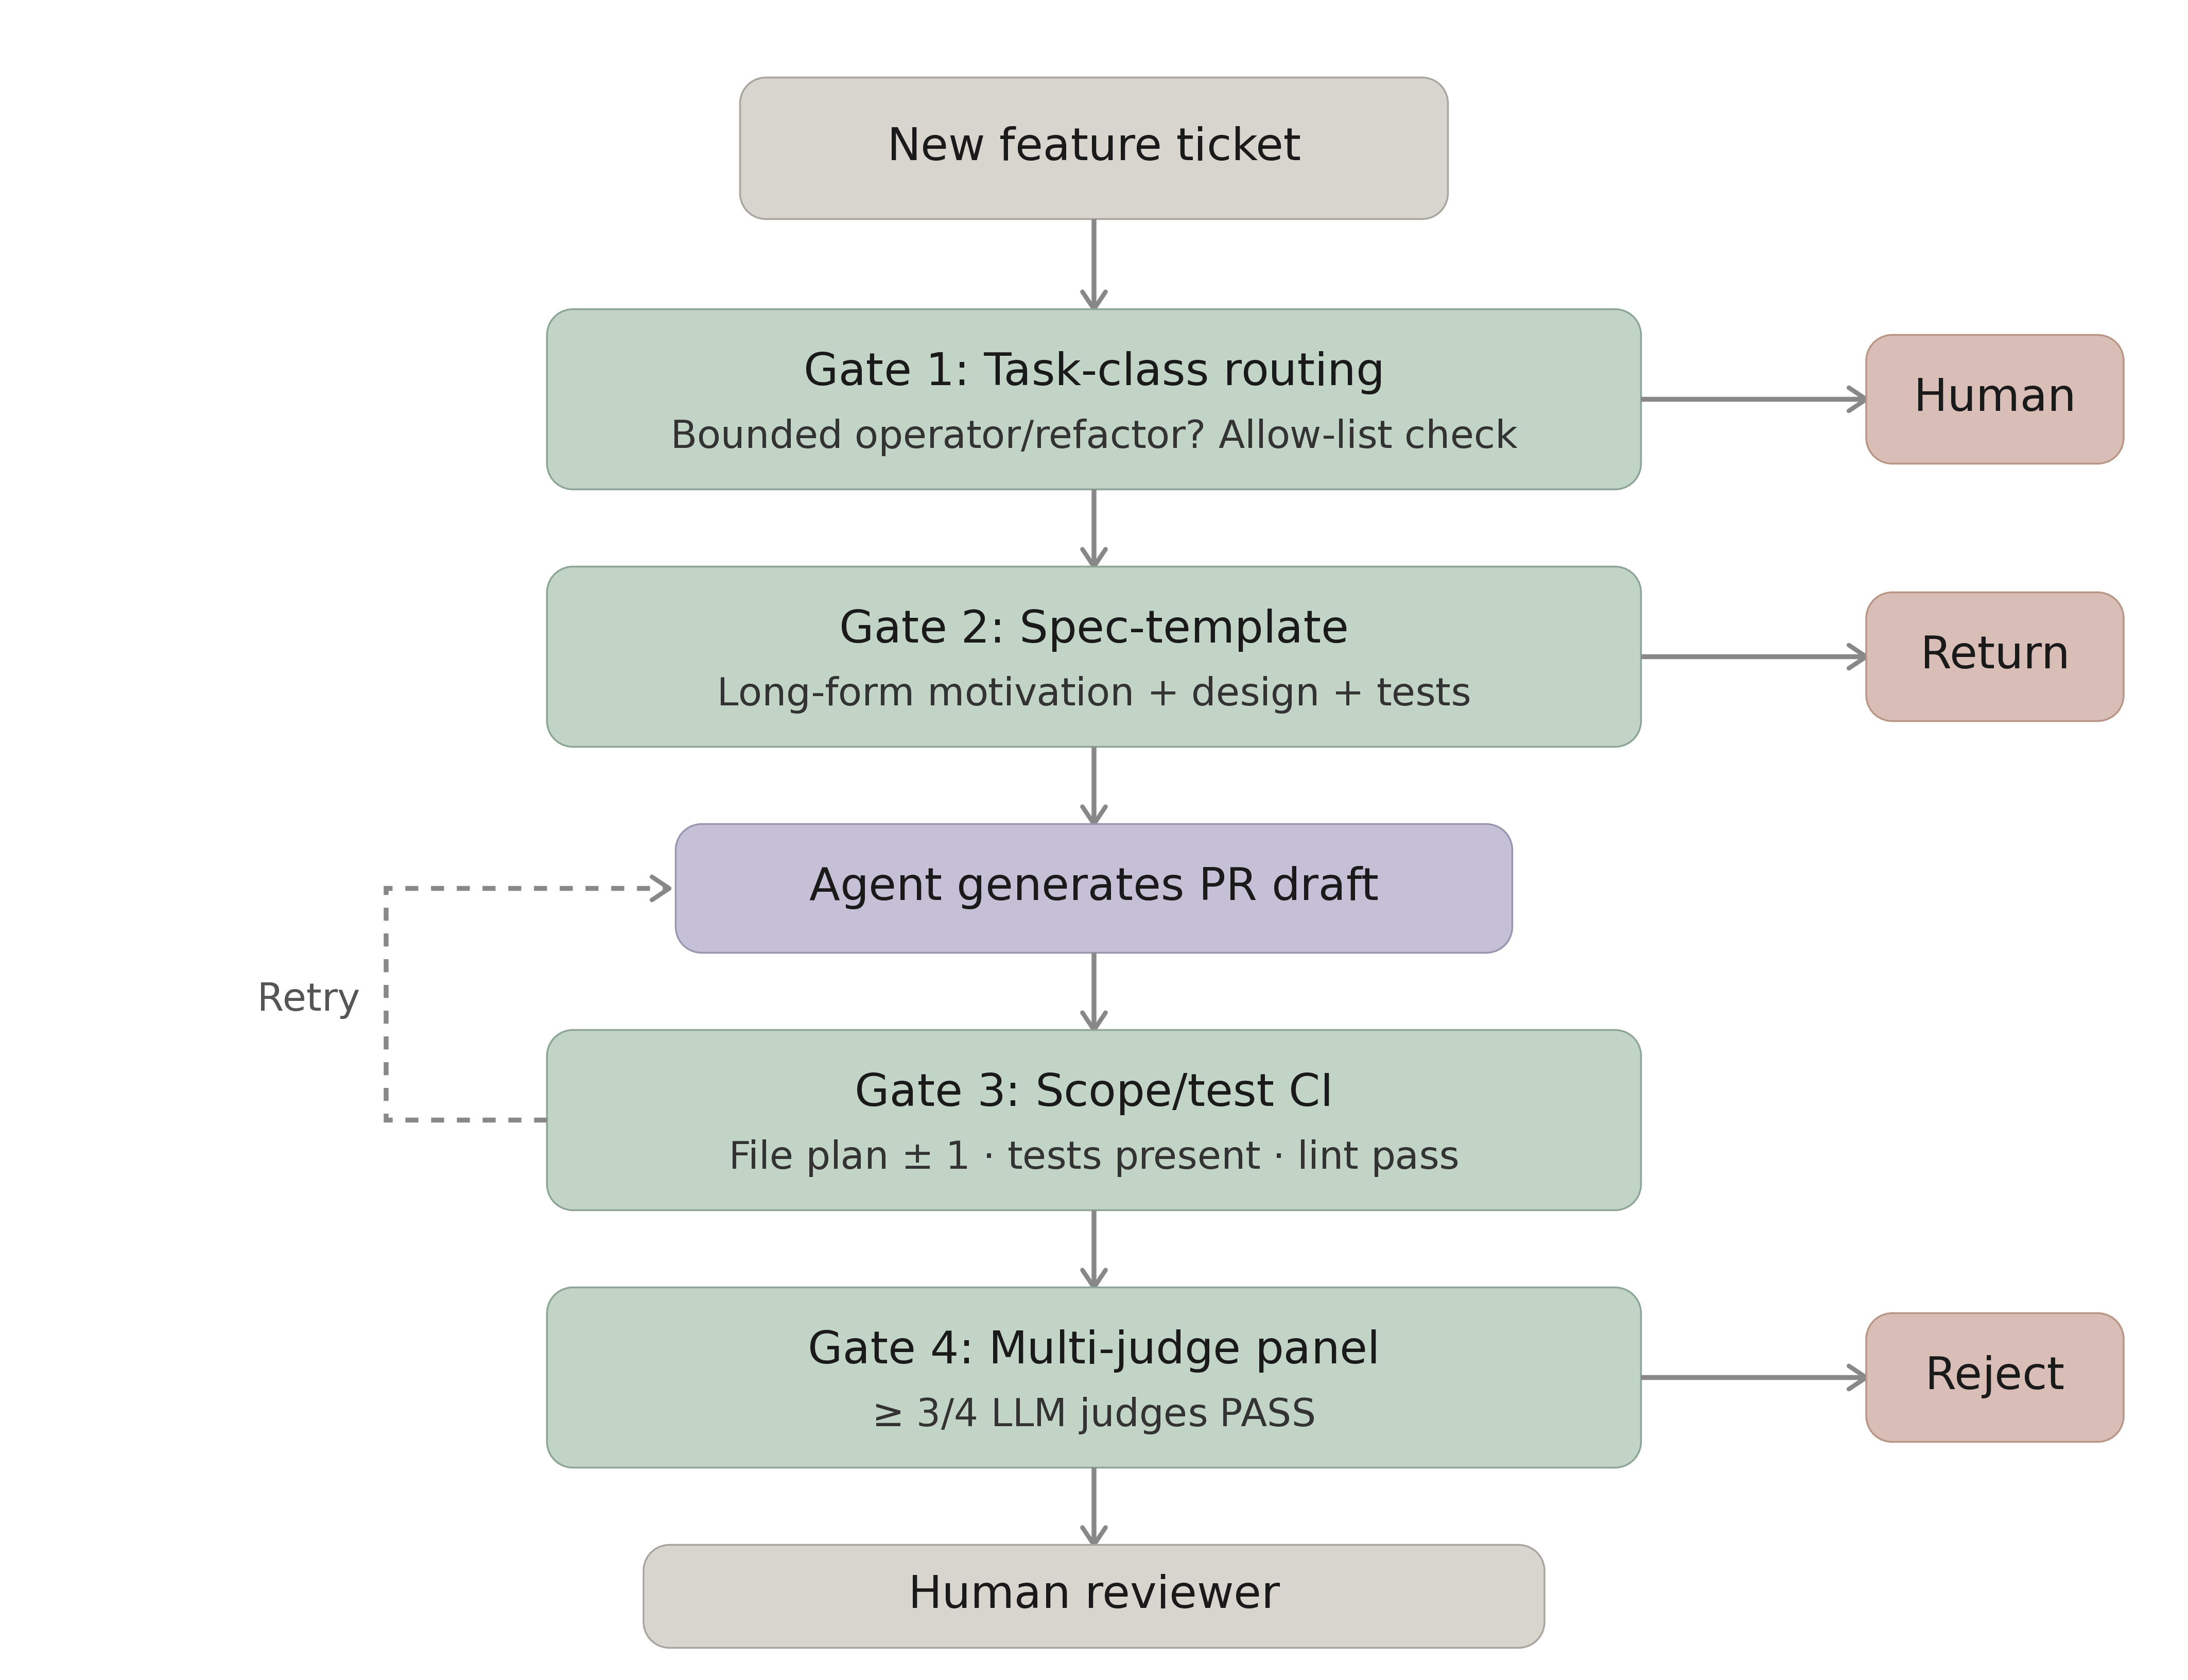
\includegraphics[width=\columnwidth]{svg/deployment_gate_pipeline.pdf}
\caption{Four-gate deployment pipeline. Each gate addresses a specific failure mode surfaced by the audit: task-class routing (0/32 Kubernetes SE-PASS), spec template (long prompts lift scores by +1.0--2.1), scope/test CI (25.5\% coverage-gap failures), and multi-judge panel (pairwise agreement as low as 42.5\%).}
\label{fig:deployment-pipeline}
\end{figure}

\paragraph{Route only bounded feature work to agents.}
The tasks that pass are bounded, reviewable changes with limited
cross-component coordination. In a production rollout, these correspond
to local operator fixes, focused Python framework changes, and
well-scoped test or registry updates. Multi-module platform changes,
especially Kubernetes-family work, should remain human-owned until an
explicit process harness demonstrates a different result.

\paragraph{Treat task specification as an engineering artifact.}
On the main corpus, long prompts lift mean composite scores by
$+1.0$ to $+2.1$ across all four agents (Table~\ref{tab:prompt}),
though the SE-PASS gain is confined to the trivially scoped T10.
On the calibration subset, Claude and Codex rise from 0\% to 8.3\%
SE-PASS with long prompts.
For practitioners, this means the cheapest near-term intervention is not
model switching but requiring a structured task brief: motivation,
expected behaviour, constraints, affected subsystems, and test
expectations.

\paragraph{Require scope and test gates before review.}
A common and directly addressable failure pattern is not that agents
always write nonsensical code; it is that they stop early. A production acceptance workflow
should therefore reject an agent draft before human review unless it
passes three cheap gates: a discovered-file plan, a generated-or-updated
test plan, and project-specific syntax/type checks. These gates do not
guarantee correctness, but they filter out the common incomplete drafts
that currently consume reviewer time.

\paragraph{Use evaluator panels, not a single judge.}
Raw pairwise agreement spans 42.5\% (Codex vs.\ GLM) to 74.4\%
(Claude vs.\ Cursor), and Fleiss' $\kappa$ is only 0.30. Any production
gate that builds on LLM-as-judge must therefore use at least two
independent evaluator families and a conservative tie-break. Single
judge gates will drift simply by swapping the judge model.

\paragraph{Separate offline evaluation from online rollout.}
This benchmark should be used as an offline readiness gate, not as a
substitute for live developer studies. A team can first run the same
task families through candidate agents, then admit only task classes
whose SE-PASS and PARTIAL rates justify reviewer time, and finally measure
acceptance rate and review burden in a controlled pilot.

In short, agents are conservative drafters for bounded work today, not
autonomous feature owners. The investment that converts the 1.0\%
main-corpus SE-PASS rate (0.0\% excluding trivially scoped tasks) into
something deployable is harness engineering: forcing scope discovery,
test evidence, and multi-judge acceptance \emph{before} a human reviewer
ever sees the change.

\begin{figure}[t]
  \centering
  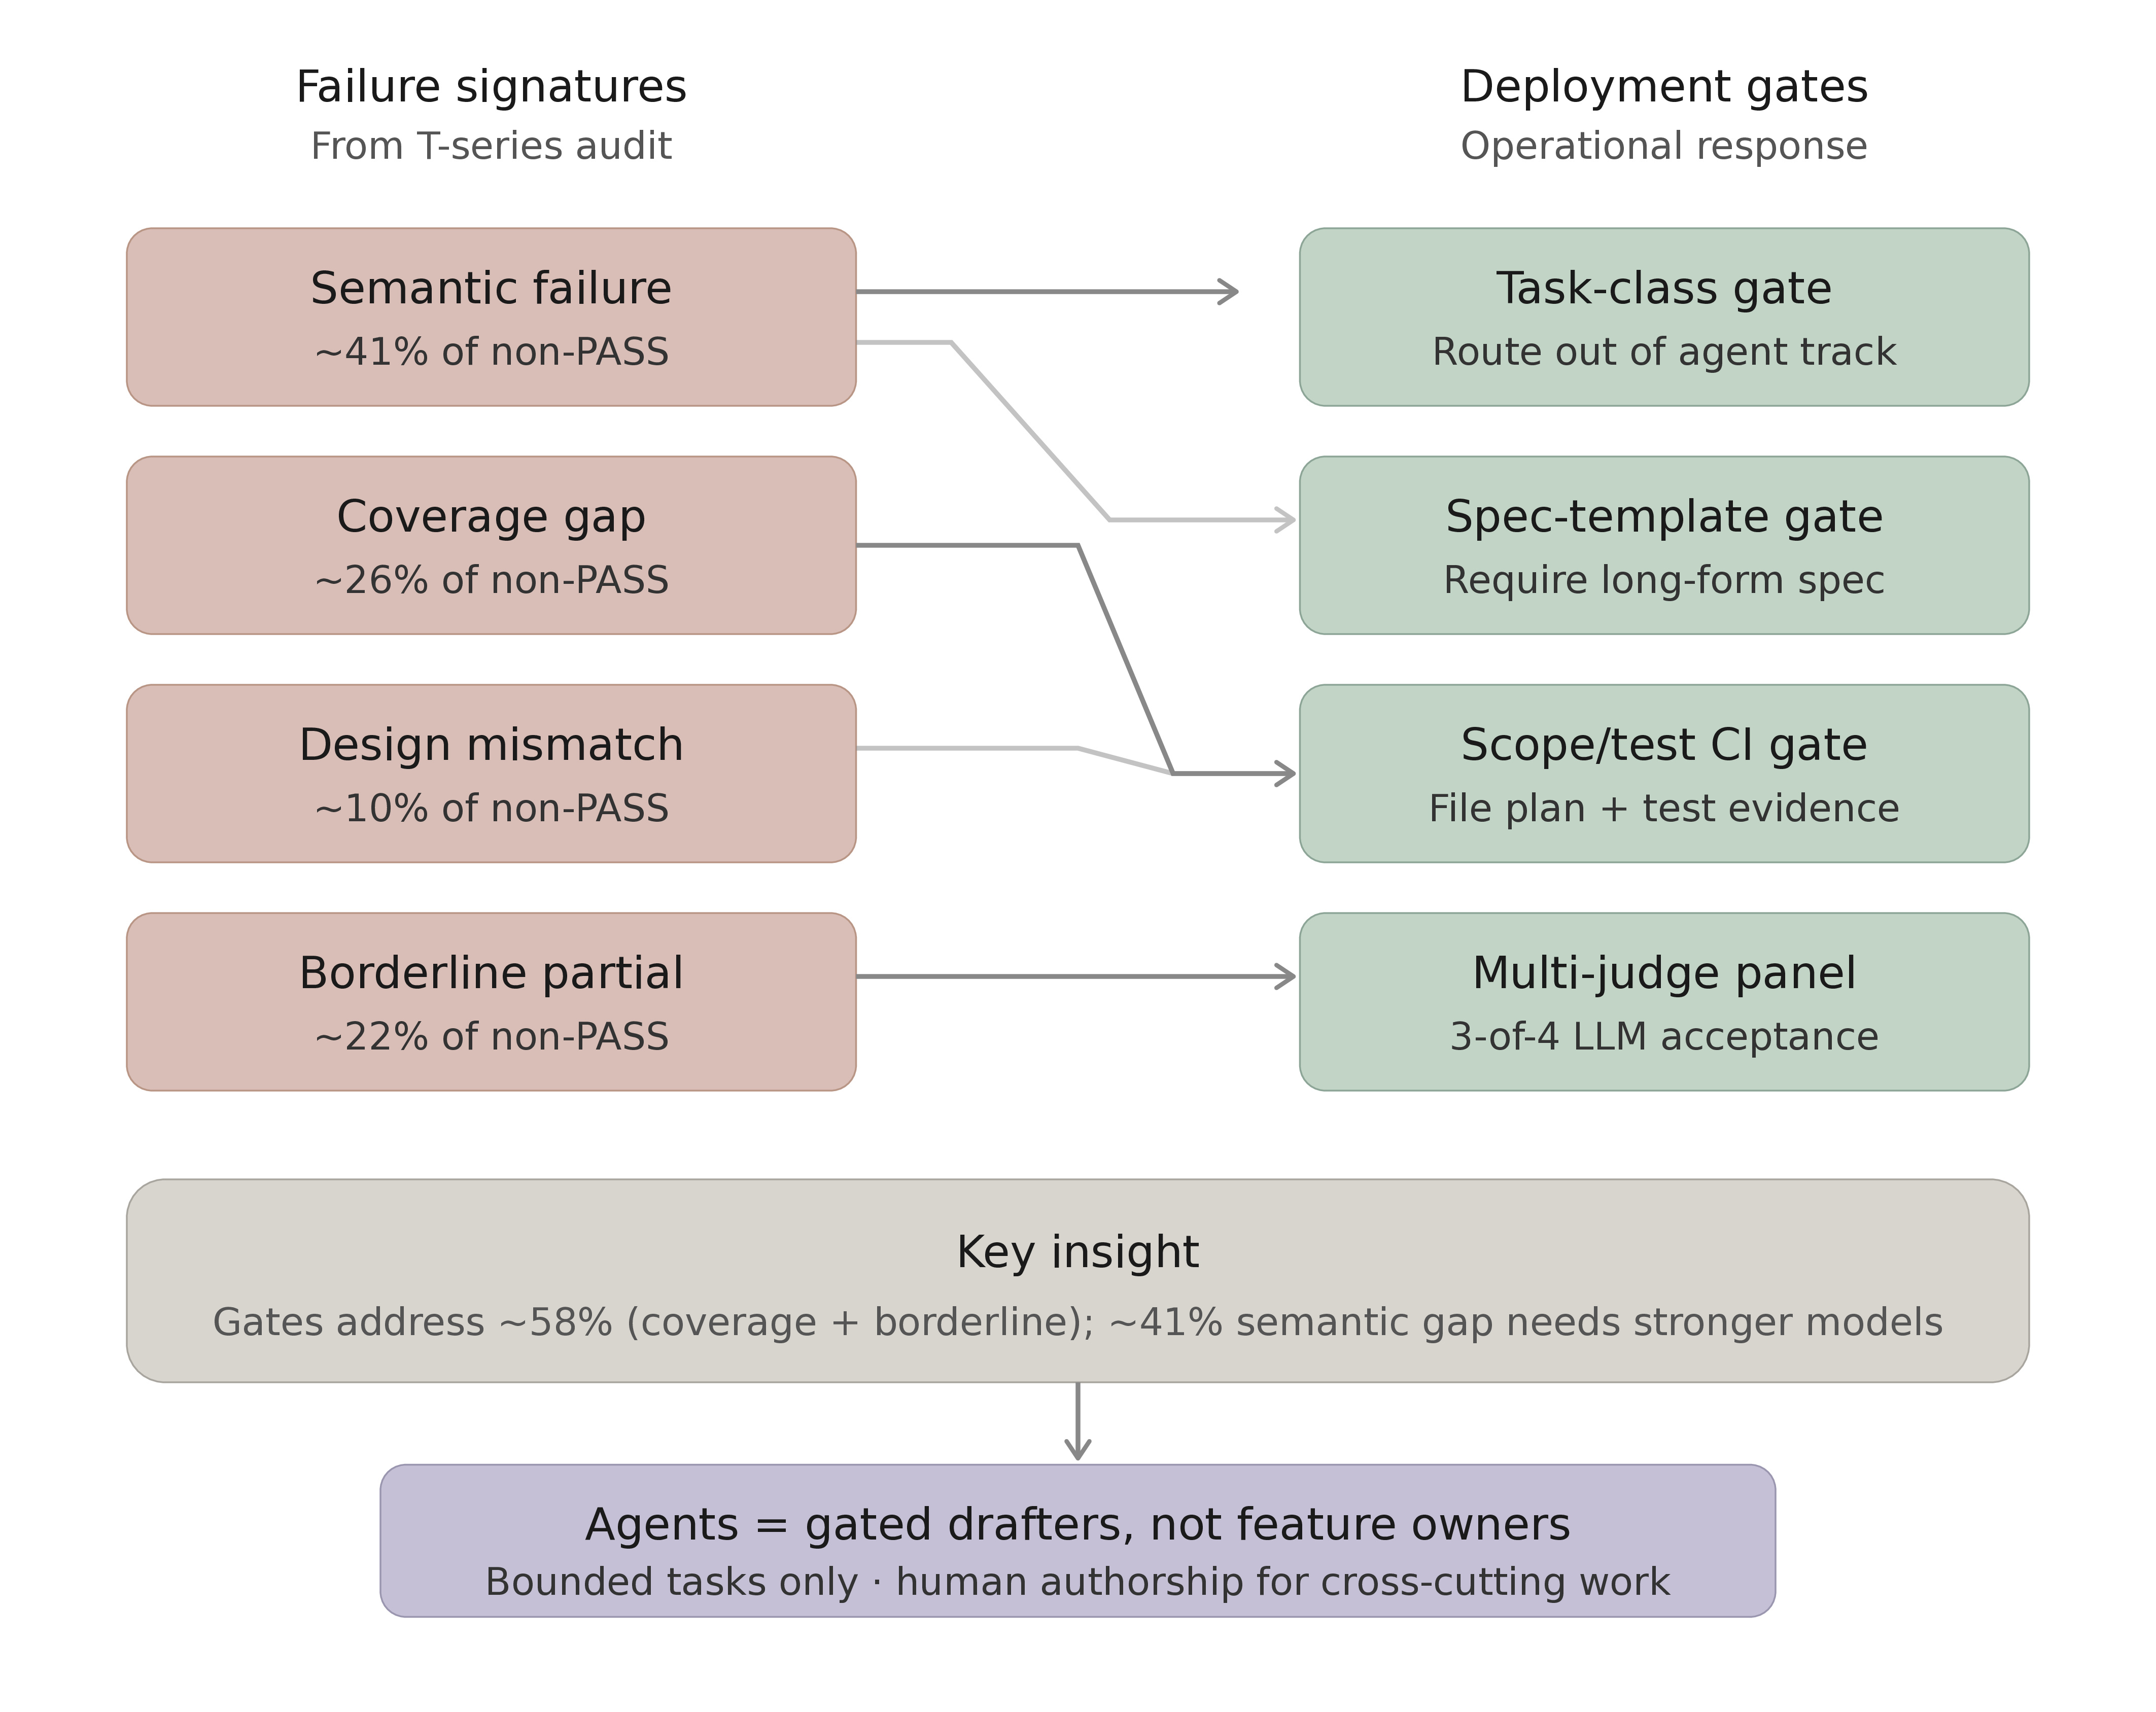
\includegraphics[width=0.9\columnwidth]{svg/failure_to_gate_mapping.pdf}
  \caption{Mapping from failure signatures (\S\ref{sec:root-cause}) to deployment gates. Coverage gaps and borderline partials (44.4\% combined) are directly filterable; the semantic-failure slice (44.7\%) requires model or specification improvements beyond current gating.}
  \label{fig:failure-gate-map}
\end{figure}

\paragraph{Deployment decision flow.}
The four interventions above compose into a single routing pipeline
that every agent-eligible feature ticket must clear before reaching a
human reviewer:
\begin{enumerate}\itemsep0pt
  \item \emph{Task-class gate.} Lookup against an allow-list (today:
    bounded operator/MindSpore-style refactors); Kubernetes-class and
    cross-module API changes route to human authoring directly.
  \item \emph{Spec-template gate.} The long-form template is mandatory
    for agent invocation; tickets without motivation, behavior, scope,
    and tests are returned to the requester.
  \item \emph{Pre-review CI gate.} The agent's PR must (a) match the
    declared file scope within $\pm$1, (b) include or update the
    declared tests, and (c) pass language-server diagnostics. Failures
    return to the agent for self-repair (bounded retry).
  \item \emph{Multi-judge acceptance.} The four-LLM panel from this
    paper runs as a pre-merge check; only $\geq 3/4$ SE-PASS is forwarded
    to human review.
\end{enumerate}
The pipeline turns the 1.0\% unconditional main-corpus SE-PASS rate into
a useful operating point: agents draft, gates filter, and human reviewers
see only candidates that already pass coverage, structure, and judge
checks. The audit's empirical contribution is precisely to identify which
gates remove the non-SE-PASS draft mass observed in §\ref{sec:results}.

\paragraph{What changed for Huawei's rollout after this audit.}
The audit produced four operational decisions inside Huawei's coding-agent
rollout. \emph{(i) Allow-list by task family.} Operator-tier CANN/MindSpeed
work is approved for agent-first drafting; Kubernetes-class control-plane
work is held back pending harness gates. \emph{(ii) Mandatory long-form
specification.} Every agent-eligible ticket now ships with the same
\emph{motivation/design-detail/test-expectation} structure used for the
\textsf{long} prompts in this study, because it is the only condition
under which we measured non-trivial SE-PASS. \emph{(iii) Pre-review CI gate.}
The two recurring failure modes (incomplete file plan and missing test
evidence) are rejected before a draft reaches a human reviewer.
(iv) \emph{Multi-judge acceptance.} A 3-of-4 LLM-judge panel, calibrated
against the same human-rater set used in this paper, is run on every
agent PR before merge.
